\documentclass[a4paper]{article}

\usepackage[english]{babel}
\usepackage[utf8]{inputenc}
\usepackage{amsmath}
\usepackage{graphicx}
\usepackage[colorinlistoftodos]{todonotes}
\usepackage[T1]{fontenc}	%ADDED for << og >>
\usepackage{enumitem}		%ADDED for smaller spacing


\title{Assinment36}
\author{pebj, smot}
\date{\today}

\begin{document}
\maketitle
	
	\begin{figure}
		\centering
		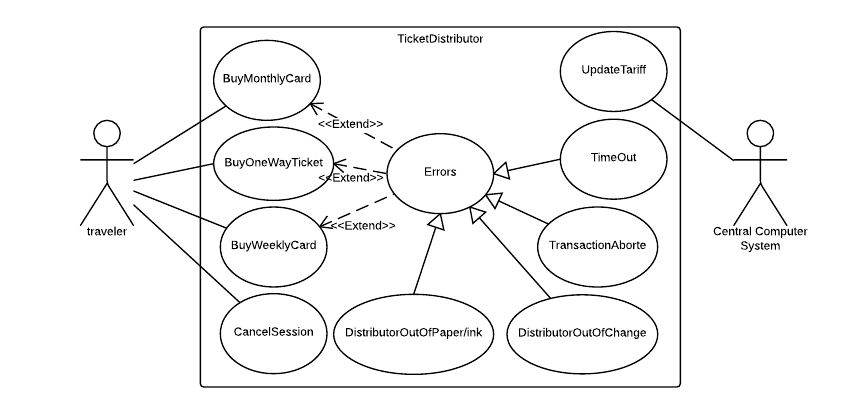
\includegraphics[width=1.3\textwidth]{UseCaseDiagram.png}\\
		\caption{\textbf{A UML} use case diagram for TicketDistributor, describing the functionality of a ticket distributor. The actor \textit{traveler} can chose between 3 differen Ticket types (with \textbf{BuyMonthlyCard}, \textbf{BuyOneWayTicket} and \textbf{BuyWeeklyCard} use cases) and cancel his progras at any point(with \textbf{CancelSession} use case). But only the \textit{Central Computer System} actor can update the tickets (with the \textbf{UpdateTariff} use case). All the Ticket type use cases Extends the \textbf{Errors} use case because thay have to test for the different errors to make sure the session is successful.}
		\label{Usecase}
	\end{figure}
	
	\begin{figure}
		\centering
		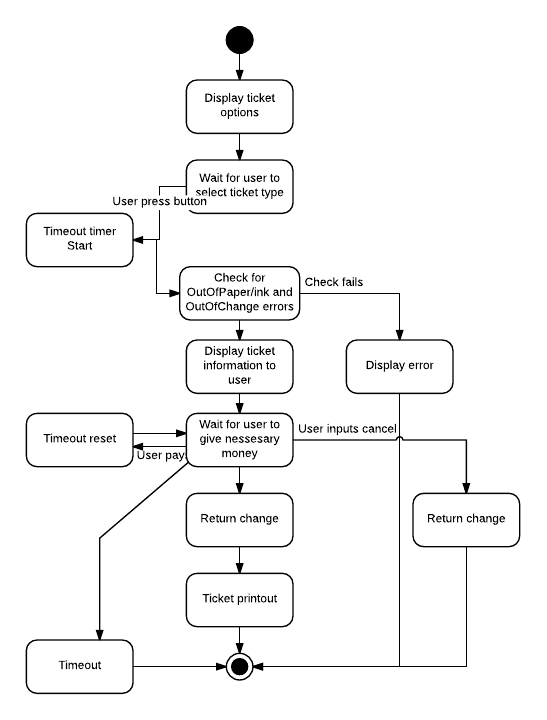
\includegraphics[width=1\textwidth]{ActivityDiagram.png}\\
		\caption{\textbf{A UML} activity diagram for TicketDistributor.}
	\end{figure}
	
	\begin{figure}
		\centering
		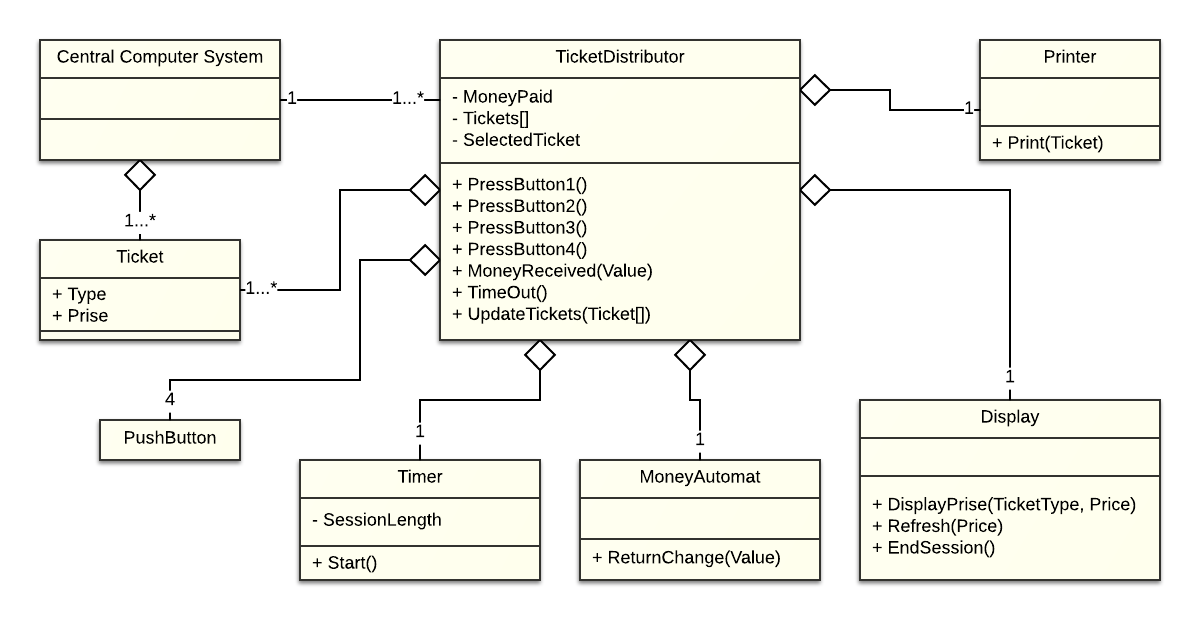
\includegraphics[width=1\textheight, angle = 270]{ClassDiagram.png}\\
		\caption{\textbf{A UML} class diagram for TicketDistributor.}
	\end{figure}
	
	\begin{figure}
		\centering
		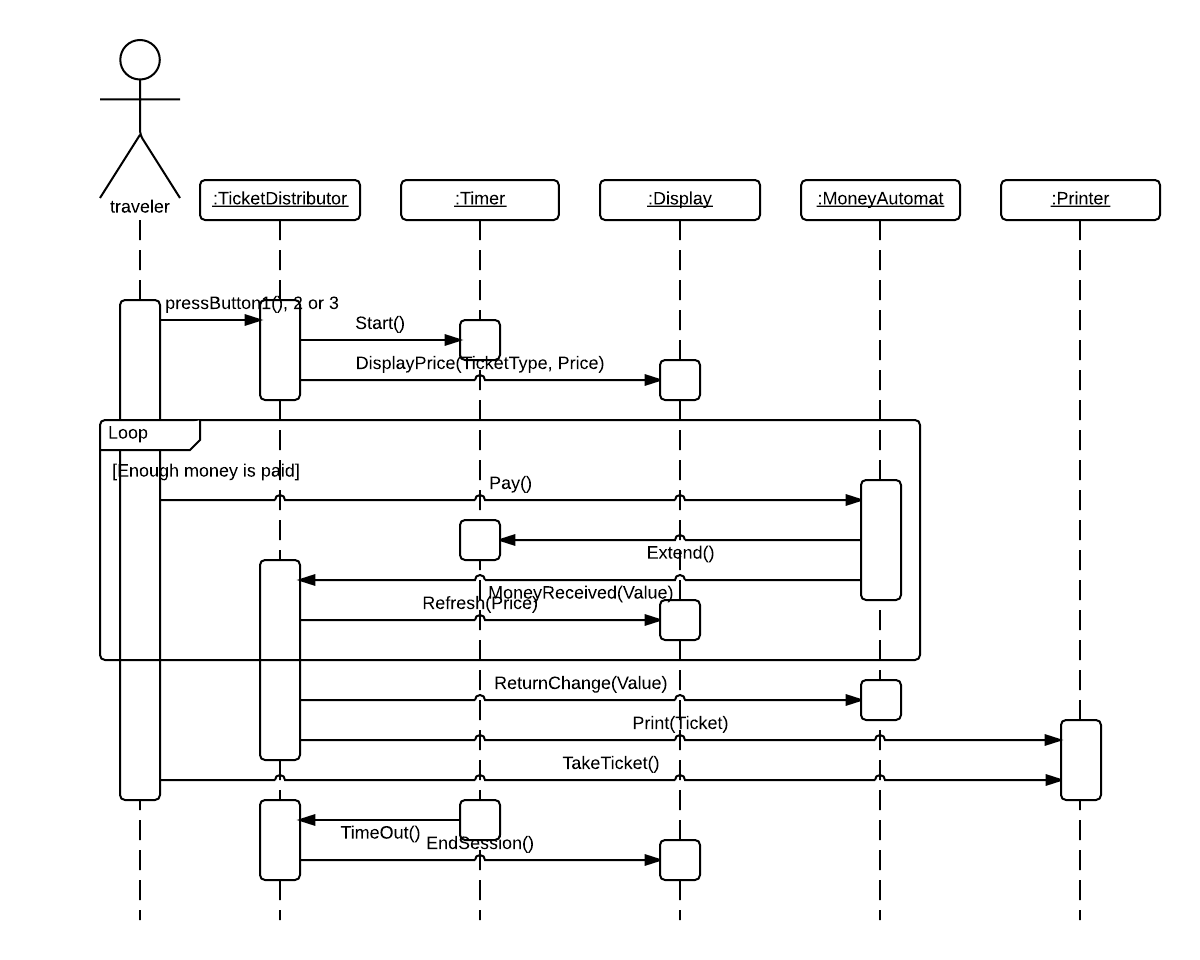
\includegraphics[width=0.95\textheight, angle = 270]{SequenceDiagram.png}\\
		\caption{\textbf{A UML} sequence diagram for the use cases BuyMonthlyCard, BuyOneWayTicket and BuyWeeklyCard, seen in Figure \ref{Usecase}.}
	\end{figure}

\end{document}